%%%%%%%%%%%%%%%%%%%%%%%%%%%%%%%%%%%%%%%%%
% Jacobs Landscape Poster
% LaTeX Template
% Version 1.0 (29/03/13)
%
% Created by:
% Computational Physics and Biophysics Group, Jacobs University
% https://teamwork.jacobs-university.de:8443/confluence/display/CoPandBiG/LaTeX+Poster
%
% Further modified by:
% Nathaniel Johnston (nathaniel@njohnston.ca)
%
% Modified further still by:
% Abraham Nunes (nunes <at> dal <dot> ca)
%
% License:
% CC BY-NC-SA 3.0 (http://creativecommons.org/licenses/by-nc-sa/3.0/)
%
%%%%%%%%%%%%%%%%%%%%%%%%%%%%%%%%%%%%%%%%%

%----------------------------------------------------------------------------------------
%	PACKAGES AND OTHER DOCUMENT CONFIGURATIONS
%----------------------------------------------------------------------------------------

\documentclass[final,table]{beamer}
\usepackage{multirow}

\usepackage[scale=1.24]{beamerposter} % Use the beamerposter package for laying out the poster
\usepackage{array}
\usetheme{confposter} % Use the confposter theme supplied with this template
\usepackage{bm}
\usepackage{xspace}
\usepackage{mathtools}
\usepackage{bm}
\usepackage{multirow}
\usepackage{adjustbox}
\setbeamercolor{block title}{fg=black,bg=} % Colors of the block titles
\setbeamercolor{block body}{fg=black,bg=} % Colors of the body of blocks
\setbeamercolor{block alerted title}{fg=white,bg=black} % Colors of the highlighted block titles
\setbeamercolor{block alerted body}{fg=black,bg=white} % Colors of the body of highlighted blocks
% Many more colors are available for use in beamerthemeconfposter.sty

\newcommand{\deemph}[1]{{\color{black!40}#1}}

%-----------------------------------------------------------
% Define the column widths and overall poster size
% To set effective sepwid, onecolwid and twocolwid values, first choose how many columns you want and how much separation you want between columns
% In this template, the separation width chosen is 0.024 of the paper width and a 4-column layout
% onecolwid should therefore be (1-(# of columns+1)*sepwid)/# of columns e.g. (1-(4+1)*0.024)/4 = 0.22
% Set twocolwid to be (2*onecolwid)+sepwid = 0.464
% Set threecolwid to be (3*onecolwid)+2*sepwid = 0.708

\newlength{\sepwid}
\newlength{\onecolwid}
\newlength{\twocolwid}
\newlength{\threecolwid}
\setlength{\paperwidth}{48in} % A0 width: 46.8in
\setlength{\paperheight}{36in} % A0 height: 33.1in
\setlength{\sepwid}{0.024\paperwidth} % Separation width (white space) between columns
\setlength{\onecolwid}{0.22\paperwidth} % Width of one column
\setlength{\twocolwid}{0.464\paperwidth} % Width of two columns
\setlength{\threecolwid}{0.708\paperwidth} % Width of three columns
\setlength{\topmargin}{-0.5in} % Reduce the top margin size

\makeatletter
\newcommand{\srcsize}{\@setfontsize{\srcsize}{5pt}{5pt}}
\makeatother

\setbeamerfont{bibliography entry author}{size=\tiny,}
\setbeamerfont{bibliography entry title}{size=\tiny}
\setbeamerfont{bibliography entry location}{size=\tiny,}
\setbeamerfont{bibliography entry note}{size=\tiny,}
%-----------------------------------------------------------

\usepackage{graphicx}  % Required for including images

\usepackage{booktabs} % Top and bottom rules for tables
\usepackage{setspace}
\DeclarePairedDelimiter\abs{\lvert}{\rvert}%
\DeclarePairedDelimiter\norm{\lVert}{\rVert}%
%----------------------------------------------------------------------------------------
%	TITLE SECTION
%----------------------------------------------------------------------------------------

\title{Plasticity and Evolvability in a Gene Regulatory Network Model} % Poster title

\author{Matthew Moreno$^{1}$} % Author(s)

\institute{$^{1}$Michigan State University}% Institution(s)

%----------------------------------------------------------------------------------------

\begin{document}
\addtobeamertemplate{block end}{}{\vspace*{2ex}} % White space under blocks
\addtobeamertemplate{block alerted end}{}{\vspace*{2ex}} % White space under highlighted (alert) blocks

\setlength{\belowcaptionskip}{2ex} % White space under figures
\setlength\belowdisplayshortskip{2ex} % White space under equations

\begin{frame}[t] % The whole poster is enclosed in one beamer frame

\begin{columns}[t] % The whole poster consists of three major columns, the second of which is split into two columns twice - the [t] option aligns each column's content to the top

\begin{column}{\sepwid}\end{column} % Empty spacer column

\begin{column}{\onecolwid} % The first column

%----------------------------------------------------------------------------------------
%	INTRODUCTION
%----------------------------------------------------------------------------------------
\vspace{-3.5ex}
\begin{block}{Summary}
\vspace{-2.5ex}
{\small
Ant foraging behavior is a collective decision making process in which, through  pheromone deposition and individual interactions between ants, a colony of ants selects and exploits a path between their nest and a food source.
Research into the collective decision making strategies of ants, in addition to characterizing the biological mechanisms and emergent properties of the foraging process, has the potential to be leveraged into applications such as swarm robotics and commercial logistics management. Although ant foraging behavior has been extensively studied on flat terrains, ant foraging over uneven terrains is not well studied. This research presents an individual-based set of differential equations to model ant foraging behavior over uneven terrain in an enclosed arena. This model is employed to investigate the characteristics of foraging paths that ants tend towards when foraging over simple inclines of varying magnitudes. Numerical solutions of the model predict that, over most inclines, ants tend to favor the direct path between nest and food, with the direct path typically being more strongly favored when foraging over steep inclines.
}
\vspace{-0.5ex}
\begin{columns}[T, onlytextwidth]
\column{0.65\textwidth}

\includegraphics[width=\textwidth]{img/placeholder}
\column{0.05\textwidth}
\column{0.3\textwidth}
\begin{spacing}{1.0}
{\small
\textit{Tetramorium caespitum} (Photo courtesy Alexander Wild.)}
\end{spacing}
\end{columns}
\end{block}

%------------------------------------------------

%----------------------------------------------------------------------------------------
%	OBJECTIVES
%----------------------------------------------------------------------------------------


%----------------------------------------------------------------------------------------

\end{column} % End of the first column

\begin{column}{\sepwid}\end{column} % Empty spacer column

\begin{column}{\twocolwid} % Begin a column which is two columns wide (column 2)

%----------------------------------------------------------------------------------------
%	IMPORTANT RESULT
%----------------------------------------------------------------------------------------

\vspace{-3.5ex}

\begin{block}{Model Components}
\vspace{-5ex}
\begin{tabular}{*{4}{>{\centering\arraybackslash}p{0.25\textwidth}}}
\begin{centering}

\includegraphics[width=0.20\textwidth]{img/placeholder}
\end{centering} &

\includegraphics[width=0.20\textwidth]{img/placeholder} &

\includegraphics[width=0.20\textwidth]{img/placeholder} & 

\includegraphics[width=0.20\textwidth]{img/placeholder} \\
\begin{spacing}{1.0}
\raggedright{\small
\textbf{Constant Power Propulsion} ants move fastest on slight decline}
\end{spacing} &
\begin{spacing}{1.0}
\raggedright{\small
\textbf{Food Attraction} magnitude increases exponentially with proximity to food}
\end{spacing} &
\begin{spacing}{1.0}
\raggedright{\small
\textbf{Nest Attraction} returner ant accelerates towards nest with constant magnitude}
\end{spacing} &
\begin{spacing}{1.0}
\raggedright{\small
\textbf{Near Nest Attraction} magnitude increases with nest proximity; acts $\perp$ to heading}
\end{spacing}
\\[-1.5cm]

\includegraphics[width=0.20\textwidth]{img/placeholder} &

\includegraphics[width=0.20\textwidth]{img/placeholder} &

\includegraphics[width=0.20\textwidth]{img/placeholder} &

\includegraphics[width=0.20\textwidth]{img/placeholder} \\
\begin{spacing}{1.0}
\raggedright{\small
\textbf{Role Switching} occurs 1cm from food (forager $\rightarrow$ returner) or nest (returner $\rightarrow$ forager)}
\end{spacing} &
\begin{spacing}{1.0}
\raggedright{\small
\textbf{Pheromone Deposit} rate proportional to ant speed (i.e. uniform per unit distance)}
\end{spacing} &
\begin{spacing}{1.0}
\raggedright{\small
\textbf{Pheromone Response} difference in pheromone between L and R determines magnitude}
\end{spacing} &
\begin{spacing}{1.0}
\raggedright{\small
\textbf{Pheromone Evaporation} rate proportional to pheromone concentration}
\end{spacing} \\[-1.5cm]

\includegraphics[width=0.20\textwidth]{img/placeholder} &

\includegraphics[width=0.20\textwidth]{img/placeholder} &

\includegraphics[width=0.20\textwidth]{img/placeholder} &

\includegraphics[width=0.20\textwidth]{img/placeholder} \\
\begin{spacing}{1.0}
\raggedright{\small
\textbf{``Boltzmann walker''} ant heading modified at occasional random reorientation events}
\end{spacing} &
\begin{spacing}{1.0}
\raggedright{\small
\textbf{Reorientation on Incline} random reorientation biased to alignments parallel to gradient}
\end{spacing} &
\begin{spacing}{1.0}
\raggedright{\small
\textbf{Arena Terrain} comprised of two flat sections joined by a simple incline}
\end{spacing} &
\begin{spacing}{1.0}
\raggedright{\small
\textbf{Nest/Food Placement} center-to-center shown in orange, corner-to-corner shown in purple}
\end{spacing} \\
\end{tabular}
\end{block}


%----------------------------------------------------------------------------------------
\vspace{-6ex}
\begin{columns}[t,totalwidth=\twocolwid] % Split up the two columns wide column again

\begin{column}{\onecolwid} % The first column within column 2 (column 2.1)


%----------------------------------------------------------------------------------------

\end{column} % End of column 2.1

\begin{column}{\onecolwid} % The second column within column 2 (column 2.2)


\end{column} % End of column 2.2

\end{columns} % End of the split of column 2

\end{column} % End of the second column

\begin{column}{\sepwid}\end{column} % Empty spacer column

\begin{column}{\onecolwid} % The third column
\vspace{-3.5ex}
\begin{block}{Conclusion}
\vspace{-2.5ex}
\small{
The relationship between evolvability and environmental influence on the phenotype was investigated using digital experiments performed on a genetic regulatory model.
The capacity of the model to accommodate the emergence of direct, indirect, and combined plasticity in evolved genetic regulatory networks was confirmed.
The phenotypic response of champion individuals evolved under regimes of direct plasticity and indirect plasticity was assessed.
The model predicts that direct plasticity and indirect plasticity decrease and increase the frequency of silent mutations, respectively.
The model also predicts that combined plasticity induces an increase in the frequency of phenotypically-expressed non-lethal mutation without having a noticeable effect on the observed frequency of silent mutation.

These experimental results confirm the existence of a relationship between phenotypic plasticity and evolvability.
It is hypothesized that this relationship is mediated by internal structural characteristics of the evolved gene regulatory networks.
Specifically, it is postulated that environmental influence on the phenotype induces selection for certain internal characteristics that support direct and/or indirect plasticity which, in turn, affect the outcome of mutation.
The exact nature of internal structural characteristics that support direct and indirect plasticity remains unknown.
Analysis of the outcome of mutation of champion individuals evolved under a combined plasticity regime in comparison to individuals evolved under just a direct plasticity regime and just an indirect plasticity regime suggests that direct and indirect plasticity stem from different aspects of internal structural configuration. 
Further work is called for to pin down a structural characterization of the internal characteristics that support direct and indirect plasticity in order to investigate the hypothesized nature of the relationship between evolvability and phenotypic plasticity.
}
\end{block}


%----------------------------------------------------------------------------------------
%	REFERENCES
%----------------------------------------------------------------------------------------
\vspace{-3ex}
\begin{block}{References}
\vspace{-2.5ex}
{\tiny\bibliographystyle{abbrv}
\bibliography{Mendeley}}
\end{block}

%----------------------------------------------------------------------------------------
%	ACKNOWLEDGEMENTS
%----------------------------------------------------------------------------------------
\vspace{-3.5ex}

\begin{block}{Acknowledgements}
\vspace{-2.5ex}
\begin{spacing}{1.0}
\scriptsize{\rmfamily{
\begin{block}{Acknowledgement}
{\footnotesize
Thank you Dr. America Chambers,	Dr. Adam Smith, Dr. Brad Richards, and Dr. Charles Ofria for your mentorship and feedback.
Thanks also to the authors of the Distributed Evolutionary Algorithms in Python and Scalable Concurrent Operations in Python packages.\par
}
\end{block}
}}
\end{spacing}
\end{block}


\end{column} % End of the third column

\end{columns} % End of all the columns in the poster
\vspace{-1ex}
\deemph{
\noindent\makebox[\paperwidth]{\rule{1.1\paperwidth}{5pt}}}
\vspace{-3.5ex}

\begin{block}{Preliminary Results}
\begin{alertblock}{Direct Plasticity}
\begin{figure}
    \centering
    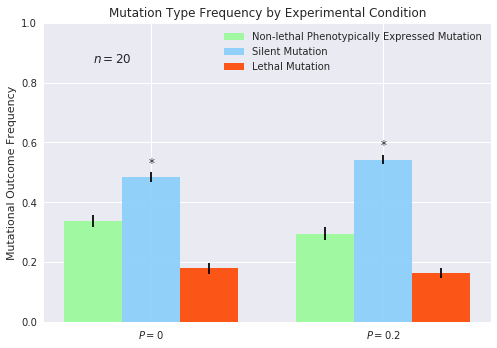
\includegraphics[width=\textwidth]{img/mutation_type_direct}
  	\caption{Champions evolved under a regime with initial state perturbation experience a higher rate of silent mutational outcomes.}
    \label{fig:mutation_type_direct}
\end{figure}
\end{alertblock}
\begin{alertblock}{Indirect Plasticity}
\begin{figure}
    \centering
    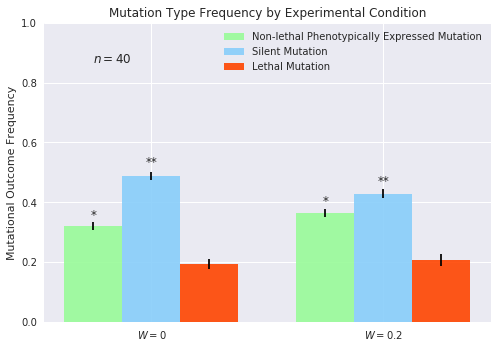
\includegraphics[width=\textwidth]{img/mutation_type_indirect}
  	\caption{Champions evolved with both primary and secondary condition/objective pairs experience a lower rate of silent mutational outcomes and a higher rate of nonlethal phenotypically observed mutational outcomes.}
    \label{fig:mutation_type_indirect}
\end{figure}
\end{alertblock}
\end{block}


\end{frame} % End of the enclosing frame

\end{document}
